\section{Radian Measure}
So far we have worked with degrees and we know that one complete revolution is $360^{\circ}$. In calculus however we will use radians. A radian is defined as the angle subtended at the center of a circle by an arc equal in length to the radius of the circle. This is illustrated in the figure below.

\begin{align*}
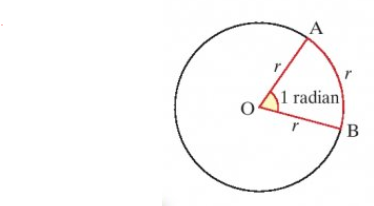
\includegraphics[scale=1]{algebra-pre-calculus/trigonometry/radian-measure/radian_measure.png}
\end{align*}


\subsection{Converting between degrees and radians}
We know that: $$ 2\pi \text{ radians} = 360^{\circ} $$
Therefore: $$ 1 \text{ radian} = \frac{360^{\circ}}{2\pi} = \frac{180^{\circ}}{\pi} $$
Conversely: $$ 1^{\circ} = \frac{2\pi}{360} = \frac{\pi}{180} \text{ radians} $$
We can write our conversions then: 
$$ 30^{\circ} = \frac{\pi}{180} \cdot 30 = \frac{\pi}{6} \text{ radians} $$
$$ 45^{\circ} = \frac{\pi}{180} \cdot 45 = \frac{\pi}{4} \text{ radians} $$
$$ 60^{\circ} = \frac{\pi}{180} \cdot 60 = \frac{\pi}{3} \text{ radians} $$
$$ 90^{\circ} = \frac{\pi}{180} \cdot 90 = \frac{\pi}{2} \text{ radians} $$
$$ 120^{\circ} = \frac{\pi}{180} \cdot 120 = \frac{2\pi}{3} \text{ radians} $$
$$ 135^{\circ} = \frac{\pi}{180} \cdot 135 = \frac{3\pi}{4} \text{ radians} $$
$$ 150^{\circ} = \frac{\pi}{180} \cdot 150 = \frac{5\pi}{6} \text{ radians} $$
$$ 180^{\circ} = \frac{\pi}{180} \cdot 180 = \pi \text{ radians} $$
$$ 270^{\circ} = \frac{\pi}{180} \cdot 270 = \frac{3\pi}{2} \text{ radians} $$
$$ 360^{\circ} = \frac{\pi}{180} \cdot 360 = 2\pi \text{ radians} $$